
	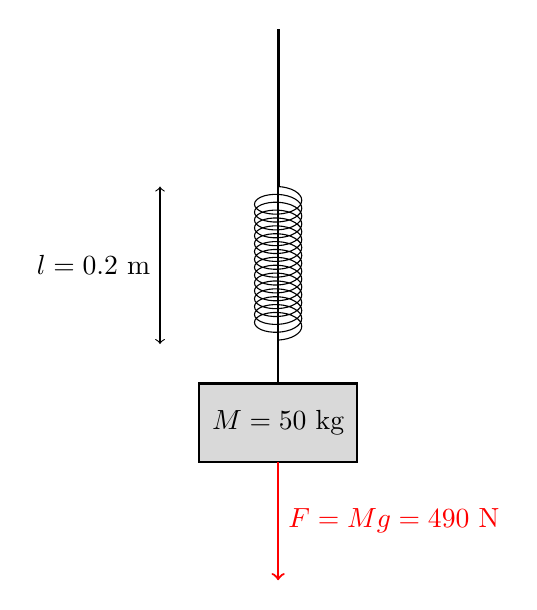
\begin{tikzpicture}
	% Draw the spring
	\draw[thick, line width=1pt] (0,0) -- (0,-2);           \draw[decorate, decoration={coil, aspect=0.5, segment length=1mm, amplitude=3mm}] (0,-2) -- (0,-4);                                                                 % Draw the mass
	\draw[thick, fill=gray!30] (-1,-4.5) rectangle (1,-5.5);                                                        \draw[thick] (0,-2) -- (0,-4.5);                                                                                % Label the mass
    \node at (0,-5) {$M = 50$ kg};                      
    % Label the spring length
	\draw[<->] (-1.5,-2) -- node[left] {$l = 0.2$ m} (-1.5,-4);                                                                                                             % Label the force arrows
	\draw[->, thick, red] (0,-5.5) -- node[right] {$F = Mg = 490$ N} (0,-7);    

	\end{tikzpicture}